% ============================================================
% CAPÍTULO 34: INTEGRALES DE SUPERFICIE Y TEOREMAS INTEGRALES
% ============================================================

\chapter{Integrales de superficie y teoremas integrales}
%%==========================================================
\section{Teorema de Green}
%%==========================================================

El teorema de Green establece una conexión entre una integral de línea
sobre una curva cerrada simple y una integral doble sobre la región
encerrada por esa curva. Es el primer resultado que relaciona el
comportamiento de un campo \emph{en el interior} de una región con su
comportamiento \emph{en la frontera}, y constituye el germen de los
teoremas de Stokes y de la divergencia que se estudiarán en la lección
siguiente.

\begin{definition}[Curva cerrada simple y orientación positiva]
Una curva $C$ en el plano se dice \textbf{cerrada} si su punto inicial
coincide con su punto final, y \textbf{simple} si no se intersecta a sí
misma (excepto en los extremos). Su \textbf{orientación positiva} es
aquella en la que la región encerrada queda siempre a la izquierda al
recorrer la curva (sentido antihorario para una curva que encierra una
región convexa).
\end{definition}

\begin{figure}[H]
\centering
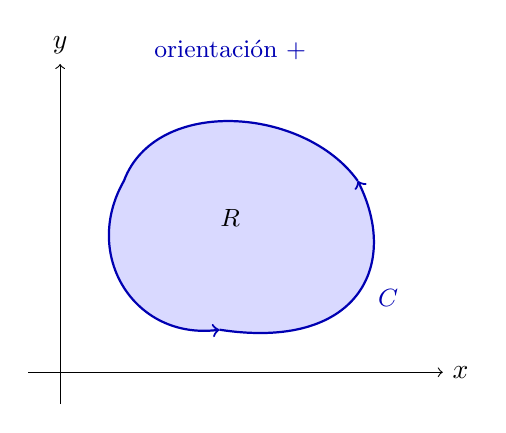
\begin{tikzpicture}[scale=1.35]
    \draw[thin,->] (-0.3,0)--(3.6,0) node[right]{$x$};
    \draw[thin,->] (0,-0.3)--(0,2.9) node[above]{$y$};
    \fill[blue!15]
        (1.5,0.4) ..controls (2.8,0.2) and (3.2,1.0).. (2.8,1.8)
                  ..controls (2.3,2.5) and (0.9,2.6).. (0.6,1.8)
                  ..controls (0.2,1.1) and (0.7,0.3).. (1.5,0.4);
    \draw[blue!70!black,thick,->]
        (1.5,0.4) ..controls (2.8,0.2) and (3.2,1.0).. (2.8,1.8);
    \draw[blue!70!black,thick,->]
        (2.8,1.8) ..controls (2.3,2.5) and (0.9,2.6).. (0.6,1.8)
                  ..controls (0.2,1.1) and (0.7,0.3).. (1.5,0.4);
    \node[blue!70!black, anchor=west] at (2.9,0.7){\small $C$};
    \node[anchor=center] at (1.6,1.45){\small $R$};
    \node[blue!70!black, font=\small, anchor=south] at (1.6,2.85){orientación $+$};
\end{tikzpicture}
\caption{Orientación positiva de $C$: la región $R$ queda siempre a la
         izquierda; la curva se recorre en sentido antihorario}
\label{fig:curva_orientacion_positiva}
\end{figure}

\begin{theorem}[Teorema de Green]
Sea $C$ una curva suave por partes, cerrada simple, orientada
positivamente en el plano, y sea $R$ la región encerrada por $C$.
Si $M(x,y)$ y $N(x,y)$ son funciones con derivadas parciales continuas
en una región abierta que contiene a $R$, entonces
\[
\oint_C M\,dx + N\,dy
= \iint_R \left( \frac{\partial N}{\partial x} - \frac{\partial M}{\partial y} \right) dA.
\]
Equivalentemente, si $\mathbf{F} = \langle M, N \rangle$,
\[
\oint_{\partial R} \mathbf{F} \cdot d\mathbf{r}
= \iint_R (\nabla \times \mathbf{F}) \cdot \mathbf{k} \, dA,
\]
donde $\nabla \times \mathbf{F} = \left( \frac{\partial N}{\partial x}
- \frac{\partial M}{\partial y} \right) \mathbf{k}$ es la componente
$z$ del rotacional.
\end{theorem}

\begin{proof}[Demostración pedagógica para regiones simples]
Basta demostrar el teorema para una región que se pueda describir
simultáneamente como una región de tipo I y de tipo II. Supóngase que
$R = \{(x,y) \mid a \le x \le b,\ g_1(x) \le y \le g_2(x)\}$. La
frontera se compone de cuatro curvas. Para la integral de $M\,dx$,
se usa el teorema fundamental del cálculo:
\[
\oint_C M\,dx
= \int_{C_1} M\,dx + \int_{C_2} M\,dx
= \int_a^b M(x,g_1(x))\,dx - \int_a^b M(x,g_2(x))\,dx,
\]
donde $C_1$ es la frontera inferior y $C_2$ la superior (orientadas
correctamente). Por el teorema fundamental,
\[
\int_{g_1(x)}^{g_2(x)} \frac{\partial M}{\partial y}\,dy
= M(x,g_2(x)) - M(x,g_1(x)).
\]
Por tanto,
\[
\oint_C M\,dx = - \int_a^b \int_{g_1(x)}^{g_2(x)}
\frac{\partial M}{\partial y}\,dy\,dx
= -\iint_R \frac{\partial M}{\partial y}\,dA.
\]
De manera análoga, expresando $R$ como región de tipo II
($c \le y \le d,\ h_1(y) \le x \le h_2(y)$), se obtiene
\[
\oint_C N\,dy = \iint_R \frac{\partial N}{\partial x}\,dA.
\]
Sumando ambas igualdades se obtiene la fórmula de Green.
\end{proof}

\begin{figure}[H]
\centering
\begin{tikzpicture}[scale=1.2]
  % Region R (ellipse)
  \fill[blue!10] (0,0) ellipse (2.2 and 1.5);
  % Vertical strip clipped to ellipse
  \begin{scope}
    \clip (0,0) ellipse (2.2 and 1.5);
    \fill[blue!25] (0.4,-2) rectangle (0.8,2);
  \end{scope}
  % Boundary C with counterclockwise arrows (positive orientation)
  \draw[thick, blue!70!black,
        postaction={decorate, decoration={markings,
          mark=at position 0.10 with {\arrow[blue!70!black]{stealth}},
          mark=at position 0.60 with {\arrow[blue!70!black]{stealth}}}}]
        (0,0) ellipse (2.2 and 1.5);
  % Reference x-axis
  \draw[dashed, gray!60] (-2.5,0) -- (2.5,0);
  % Strip vertical boundaries
  \draw[dashed, gray!70] (0.4,-1.7) -- (0.4,1.7);
  \draw[dashed, gray!70] (0.8,-1.7) -- (0.8,1.7);
  % dx label above strip
  \draw[stealth-stealth, gray!60] (0.4,1.68) -- (0.8,1.68) node[midway, above, black] {\small $dx$};
  % Labels
  \node[anchor=center] at (-0.5,0.4) {$R$};
  \node[blue!70!black, anchor=west] at (2.62,0.5) {$C$};
  \node[below] at (-2.2,0) {\small $a$};
  \node[below] at ( 2.2,0) {\small $b$};
  % g1 and g2 at x=0.8
  \node[right] at (0.83, 1.40) {\small $g_2(x)$};
  \node[right] at (0.83,-1.40) {\small $g_1(x)$};
  % C1 at bottom (goes right →) and C2 at top (goes left ←)
  \draw[->, thick, red!70!black] (0.4,-1.48) -- (0.8,-1.40)
        node[below right, scale=0.8] {$C_1$};
  \draw[<-, thick, red!70!black] (0.4, 1.48) -- (0.8, 1.40)
        node[above right, scale=0.8] {$C_2$};
\end{tikzpicture}
\caption{Región tipo\,I en la demostración del Teorema de Green: la franja vertical entre $g_1(x)$ y $g_2(x)$ muestra la aplicación del TFC en $y$. La orientación positiva (antihoraria) de $C$ implica que $C_1$ recorre el borde inferior $\to$ y $C_2$ el superior $\leftarrow$, originando el signo negativo en $-\iint_R \partial M/\partial y\,dA$.}
\label{fig:green_region_tipo_I}
\end{figure}

\begin{rem}
La demostración anterior supone que la región es simple (se puede
describir como tipo I y tipo II). Para regiones más generales (con
agujeros o fronteras más complejas), se descomponen en subregiones
simples y se aplica Green en cada una, sumando los resultados. Las
integrales de línea sobre los cortes internos se cancelan, dejando
únicamente la integral sobre la frontera exterior.
\end{rem}

\begin{pasos}[Aplicación del teorema de Green]
Para usar el teorema de Green:
\begin{enumerate}
    \item \textbf{Identificar $M$ y $N$.} Escribir el campo vectorial
    como $\mathbf{F}=\langle M,N \rangle$ y la integral de línea como
    $\oint_C M\,dx + N\,dy$.
    \item \textbf{Calcular el integrando de la integral doble.}
    Hallar $\displaystyle \frac{\partial N}{\partial x} -
    \frac{\partial M}{\partial y}$.
    \item \textbf{Describir la región $R$.} Identificar la región
    encerrada por $C$ y determinar sus límites de integración.
    \item \textbf{Evaluar la integral doble.} Calcular
    $\displaystyle \iint_R \left( \frac{\partial N}{\partial x} -
    \frac{\partial M}{\partial y} \right) dA$.
\end{enumerate}
\end{pasos}

%%==========================================================
\begin{example}[Verificación de Green]
Verificar el teorema de Green para el campo $\mathbf{F}(x,y) =
\langle -y, x \rangle$ y la región $R$ encerrada por el círculo
$x^2+y^2=4$.
\begin{myproof}
\textbf{Paso 1. Identificar $M$ y $N$.}
Aquí $M=-y$, $N=x$.

\textbf{Paso 2. Calcular el integrando de la integral doble.}
\[
\frac{\partial N}{\partial x} - \frac{\partial M}{\partial y}
= \frac{\partial}{\partial x}(x) - \frac{\partial}{\partial y}(-y)
= 1 - (-1) = 2.
\]

\textbf{Paso 3. Describir la región $R$.}
$R$ es el disco de radio $2$ centrado en el origen:
$R = \{(x,y) \mid x^2+y^2 \le 4\}$.

\textbf{Paso 4. Evaluar la integral doble.}
En coordenadas polares, $dA = r\,dr\,d\theta$, con $0 \le r \le 2$,
$0 \le \theta \le 2\pi$:
\[
\iint_R 2\,dA = 2 \int_0^{2\pi} \int_0^2 r\,dr\,d\theta
= 2 \cdot 2\pi \cdot \frac{4}{2} = 8\pi.
\]
Por el teorema de Green, la integral de línea sobre la frontera
orientada positivamente debe ser $8\pi$.

\textbf{Verificación directa.}
Parametrizamos la circunferencia como $\mathbf{r}(t)=\langle 2\cos t,
2\sin t \rangle$, $0 \le t \le 2\pi$. Entonces
\[
\mathbf{F}(\mathbf{r}(t)) = \langle -2\sin t, 2\cos t \rangle,
\quad \mathbf{r}'(t) = \langle -2\sin t, 2\cos t \rangle.
\]
Por tanto,
\[
\oint_C \mathbf{F}\cdot d\mathbf{r}
= \int_0^{2\pi} \langle -2\sin t, 2\cos t \rangle \cdot
\langle -2\sin t, 2\cos t \rangle \, dt
= \int_0^{2\pi} 4(\sin^2 t + \cos^2 t)\,dt
= \int_0^{2\pi} 4\,dt = 8\pi.
\]
La igualdad se cumple: $\boxed{8\pi = 8\pi}$.
\end{myproof}
\end{example}

%%==========================================================
\section{Divergencia y rotacional}
%%==========================================================

El teorema de Green introduce la cantidad $\partial N/\partial x -
\partial M/\partial y$, que es precisamente la componente $z$ del
rotacional de $\mathbf{F}$ en dos dimensiones. Para campos en
$\mathbb{R}^3$, el rotacional es un vector que mide la tendencia del
campo a \emph{girar} alrededor de un punto, mientras que la divergencia
mide la tendencia a \emph{fluir} hacia el exterior o el interior.

\begin{figure}[H]
\centering
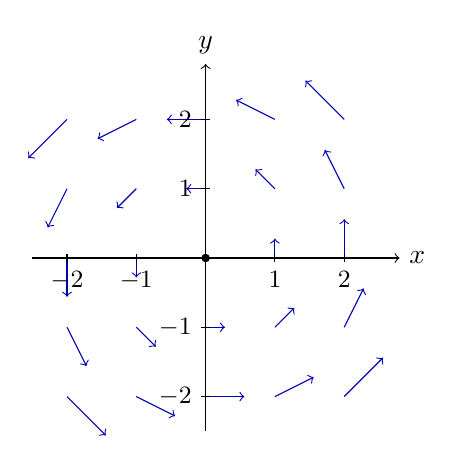
\begin{tikzpicture}[scale=0.88]
    \draw[thin,->] (-2.5,0)--(2.8,0) node[right]{$x$};
    \draw[thin,->] (0,-2.5)--(0,2.8) node[above]{$y$};
    \foreach \xi/\yi in {
        -2/-2, -2/-1, -2/0, -2/1, -2/2,
        -1/-2, -1/-1, -1/0, -1/1, -1/2,
         0/-2,  0/-1,        0/1,  0/2,
         1/-2,  1/-1,  1/0,  1/1,  1/2,
         2/-2,  2/-1,  2/0,  2/1,  2/2}{
        \draw[->,blue!70!black]
            (\xi,\yi)--({(\xi)+(-\yi)*0.28},{(\yi)+(\xi)*0.28});
    }
    \filldraw (0,0) circle (1.5pt);
    \foreach \n in {-2,-1,1,2}{
        \draw[thin] (\n,0.06)--(\n,-0.06) node[below,font=\small]{$\n$};
        \draw[thin] (0.06,\n)--(-0.06,\n) node[left,font=\small]{$\n$};
    }
\end{tikzpicture}
\caption{Campo vectorial $\mathbf{F}(x,y)=(-y,\,x)$: vectores tangentes a
         círculos concéntricos orientados en sentido antihorario
         ($\nabla\cdot\mathbf{F}=0$;\; $\nabla\times\mathbf{F}=2\mathbf{k}$)}
\label{fig:campo_vectorial_rotacional}
\end{figure}

\begin{definition}[Divergencia]
La \textbf{divergencia} de un campo vectorial $\mathbf{F}(x,y,z) =
\langle F_1, F_2, F_3 \rangle$ es el campo escalar
\[
\nabla \cdot \mathbf{F}
= \frac{\partial F_1}{\partial x}
+ \frac{\partial F_2}{\partial y}
+ \frac{\partial F_3}{\partial z}.
\]
En $\mathbb{R}^2$, para $\mathbf{F} = \langle M, N \rangle$,
\[
\nabla \cdot \mathbf{F} = \frac{\partial M}{\partial x}
+ \frac{\partial N}{\partial y}.
\]
\end{definition}

\begin{definition}[Rotacional]
El \textbf{rotacional} de un campo vectorial $\mathbf{F}(x,y,z) =
\langle F_1, F_2, F_3 \rangle$ es el campo vectorial
\[
\nabla \times \mathbf{F}
= \begin{vmatrix}
\mathbf{i} & \mathbf{j} & \mathbf{k} \\
\partial_x & \partial_y & \partial_z \\
F_1 & F_2 & F_3
\end{vmatrix}
= \left( \frac{\partial F_3}{\partial y} - \frac{\partial F_2}{\partial z} \right)
\mathbf{i}
+ \left( \frac{\partial F_1}{\partial z} - \frac{\partial F_3}{\partial x} \right)
\mathbf{j}
+ \left( \frac{\partial F_2}{\partial x} - \frac{\partial F_1}{\partial y} \right)
\mathbf{k}.
\]
En $\mathbb{R}^2$, el rotacional se reduce al escalar (componente $z$)
\[
(\nabla \times \mathbf{F}) \cdot \mathbf{k}
= \frac{\partial N}{\partial x} - \frac{\partial M}{\partial y},
\]
donde $\mathbf{F} = \langle M, N, 0 \rangle$.
\end{definition}

\begin{rem}[Interpretación física]
\begin{itemize}
    \item La \textbf{divergencia} mide la densidad de flujo neto que
    sale de un punto. Si $\nabla\cdot\mathbf{F}>0$, el punto es una
    \emph{fuente}; si es negativo, un \emph{sumidero}. Un campo
    incompresible (como el flujo de un fluido a densidad constante)
    tiene divergencia cero.
    \item El \textbf{rotacional} mide la circulación local del campo
    alrededor de un punto. Su dirección indica el eje de rotación, y
    su magnitud, la intensidad del giro. Un campo con rotacional cero
    se llama \emph{irrotacional}; si además el dominio es simplemente
    conexo, el campo es conservativo.
\end{itemize}
\end{rem}

En el contexto del teorema de Green, el integrando de la integral doble
es precisamente la componente $z$ del rotacional de $\mathbf{F}$:
\[
\nabla \times \mathbf{F} = \left( \frac{\partial N}{\partial x}
- \frac{\partial M}{\partial y} \right) \mathbf{k}.
\]
Por tanto, el teorema de Green se puede reescribir como
\[
\oint_{\partial R} \mathbf{F} \cdot d\mathbf{r}
= \iint_R (\nabla \times \mathbf{F}) \cdot \mathbf{k} \, dA,
\]
que es un caso particular en el plano del teorema de Stokes en
$\mathbb{R}^3$ (que se estudiará en la lección L4.2).

\begin{rem}[Campos conservativos y rotacional]
Un campo $\mathbf{F}$ definido en un dominio simplemente conexo es
conservativo si y solo si $\nabla \times \mathbf{F} = \mathbf{0}$
(en $\mathbb{R}^3$) o $\partial N/\partial x = \partial M/\partial y$
(en $\mathbb{R}^2$). Esta es una reformulación práctica de la condición
de simetría de las derivadas cruzadas.
\end{rem}

\begin{rem}[El teorema de Green como herramienta de cálculo]
El teorema de Green no solo es un resultado teórico: permite convertir
integrales de línea difíciles en integrales dobles más manejables, y
viceversa. También se usa para calcular áreas de regiones planas
eligiendo $\mathbf{F}$ tal que $\partial N/\partial x - \partial
M/\partial y = 1$, por ejemplo $\mathbf{F} = \langle 0, x \rangle$ o
$\mathbf{F} = \langle -y, 0 \rangle$, de modo que
\[
\text{Área}(R) = \oint_{\partial R} x\,dy = -\oint_{\partial R} y\,dx.
\]
Este es el principio del planímetro, un instrumento mecánico para medir
áreas de regiones irregulares.
\end{rem}

\begin{prob}
Calcule la integral de línea $\int_C \mathbf{F}\cdot d\mathbf{r}$ para
$\mathbf{F}(x,y)=\langle x^2, y^2 \rangle$ a lo largo de los siguientes
caminos que unen $(0,0)$ con $(1,1)$:
\begin{enumerate}[(a)]
    \item la línea recta $y=x$;
    \item la parábola $x=t$, $y=t^2$;
    \item la curva quebrada que va de $(0,0)$ a $(1,0)$ y luego a $(1,1)$.
\end{enumerate}
Compare los resultados y discuta si el campo es conservativo.
\begin{myproof}
\textbf{Paso 1. Camino (a): $y=x$.} Parametrizamos $\mathbf{r}(t)=\langle t,t\rangle$, $0\le t\le1$, $d\mathbf{r}=\langle1,1\rangle dt$. Con $\mathbf{F}=\langle t^2,t^2\rangle$:
\[
\int_{C_a}\mathbf{F}\cdot d\mathbf{r}=\int_0^1(t^2+t^2)\,dt=\frac{2}{3}.
\]
\textbf{Paso 2. Camino (b): $x=t$, $y=t^2$.} $\mathbf{r}(t)=\langle t,t^2\rangle$, $d\mathbf{r}=\langle1,2t\rangle dt$, $\mathbf{F}=\langle t^2,t^4\rangle$:
\[
\int_{C_b}\mathbf{F}\cdot d\mathbf{r}=\int_0^1(t^2+2t^5)\,dt=\frac{1}{3}+\frac{1}{3}=\frac{2}{3}.
\]
\textbf{Paso 3. Camino (c): quebrada $(0,0)\to(1,0)\to(1,1)$.}
\begin{itemize}
\item $C_1$: $\mathbf{r}=(t,0)$, $\mathbf{F}=\langle t^2,0\rangle$, $d\mathbf{r}=\langle1,0\rangle dt$;\; $\int_{C_1}=\tfrac{1}{3}$.
\item $C_2$: $\mathbf{r}=(1,t)$, $\mathbf{F}=\langle1,t^2\rangle$, $d\mathbf{r}=\langle0,1\rangle dt$;\; $\int_{C_2}=\tfrac{1}{3}$.
\end{itemize}
$\displaystyle\int_{C_c}=\frac13+\frac13=\frac{2}{3}.$

\textbf{Paso 4. Conclusión.} Los tres caminos dan $\frac23$: el campo es conservativo. Verificación: $\tfrac{\partial(y^2)}{\partial x}=0=\tfrac{\partial(x^2)}{\partial y}$ ✓. Potencial: $f(x,y)=\dfrac{x^3}{3}+\dfrac{y^3}{3}$.
\end{myproof}
\end{prob}

\begin{prob}
Determine si cada campo es conservativo. En caso afirmativo, halle su
función potencial.
\begin{multicols}{2}
\begin{enumerate}[(a)]
    \item $\mathbf{F}(x,y)=\langle 2x, 2y \rangle$
    \item $\mathbf{F}(x,y)=\langle y^2, 2xy \rangle$
    \item $\mathbf{F}(x,y)=\langle \cos y, -x\sin y \rangle$
    \item $\mathbf{F}(x,y)=\langle e^x \cos y, -e^x \sin y \rangle$
    \item $\mathbf{F}(x,y,z)=\langle 2x, 2y, 2z \rangle$
    \item $\mathbf{F}(x,y,z)=\langle yz, xz, xy \rangle$
\end{enumerate}
\end{multicols}
\begin{myproof}
Para cada campo verificamos $\partial M/\partial y=\partial N/\partial x$ (en $\mathbb{R}^2$) o $\nabla\times\mathbf{F}=\mathbf{0}$ (en $\mathbb{R}^3$); si el dominio es simplemente conexo, el campo es conservativo. Hallamos $f$ tal que $\nabla f=\mathbf{F}$.

\textbf{(a)} $\tfrac{\partial(2y)}{\partial x}=0=\tfrac{\partial(2x)}{\partial y}$ ✓.\quad $f=x^2+y^2$.

\textbf{(b)} $\tfrac{\partial(y^2)}{\partial y}=2y=\tfrac{\partial(2xy)}{\partial x}$ ✓. $\partial f/\partial x=y^2\Rightarrow f=xy^2+g(y)$;\; $\partial f/\partial y=2xy+g'=2xy\Rightarrow g'=0$. $f=xy^2$.

\textbf{(c)} $\tfrac{\partial(\cos y)}{\partial y}=-\sen y=\tfrac{\partial(-x\sen y)}{\partial x}$ ✓.\quad $f=x\cos y$.

\textbf{(d)} $\tfrac{\partial(e^x\cos y)}{\partial y}=-e^x\sen y=\tfrac{\partial(-e^x\sen y)}{\partial x}$ ✓.\quad $f=e^x\cos y$.

\textbf{(e)} $\nabla\times\langle2x,2y,2z\rangle=\mathbf{0}$ ✓.\quad $f=x^2+y^2+z^2$.

\textbf{(f)} $\mathbf{F}=\langle yz,xz,xy\rangle$: $\tfrac{\partial(xy)}{\partial y}-\tfrac{\partial(xz)}{\partial z}=x-x=0$;\; $\tfrac{\partial(yz)}{\partial z}-\tfrac{\partial(xy)}{\partial x}=y-y=0$;\; $\tfrac{\partial(xz)}{\partial x}-\tfrac{\partial(yz)}{\partial y}=z-z=0$ ✓. Integrando: $\partial f/\partial x=yz\Rightarrow f=xyz+g(y,z)$; $\partial f/\partial y=xz+\partial g/\partial y=xz\Rightarrow g=h(z)$; $\partial f/\partial z=xy+h'(z)=xy\Rightarrow h'=0$. $\boxed{f=xyz}$.
\end{myproof}
\end{prob}

\begin{prob}
Utilice el teorema fundamental de las integrales de línea para calcular
$\int_C \mathbf{F}\cdot d\mathbf{r}$ donde $\mathbf{F}(x,y) =
\langle 2xy^2, 2x^2y \rangle$ y $C$ es cualquier curva suave por partes
que une $(0,0)$ con $(1,2)$.
\begin{myproof}
\textbf{Paso 1. Verificar que $\mathbf{F}$ es conservativo.}
\[
\frac{\partial M}{\partial y}=4xy=\frac{\partial N}{\partial x}.\quad\checkmark
\]
\textbf{Paso 2. Hallar el potencial.} $\partial f/\partial x=2xy^2\Rightarrow f=x^2y^2+g(y)$;\; $\partial f/\partial y=2x^2y+g'(y)=2x^2y\Rightarrow g'=0$. Por tanto $f(x,y)=x^2y^2$.

\textbf{Paso 3. Aplicar el TFC.}
\[
\int_C\mathbf{F}\cdot d\mathbf{r}=f(1,2)-f(0,0)=1^2\cdot2^2-0=\boxed{4}.
\]
\end{myproof}
\end{prob}



\begin{prob}
Sea $R$ una región plana con frontera $C$. Demuestre que el área de $R$
está dada por
\[
A(R) = \frac{1}{2} \oint_C x\,dy - y\,dx.
\]
Use esta fórmula para calcular el área de la elipse $\frac{x^2}{a^2}
+\frac{y^2}{b^2}=1$.
\begin{myproof}
\textbf{Paso 1. Demostrar la fórmula.} Tomamos $M=-y/2$, $N=x/2$; entonces $\partial N/\partial x-\partial M/\partial y=\tfrac12+\tfrac12=1$. Por Green:
\[
\frac{1}{2}\oint_C x\,dy-y\,dx=\iint_R 1\,dA=A(R).\quad\checkmark
\]
\textbf{Paso 2. Área de la elipse.} Parametrizamos $C$: $x=a\cos t$, $y=b\sen t$, $0\le t\le2\pi$:
\[
x\,dy-y\,dx=(a\cos t)(b\cos t\,dt)-(b\sen t)(-a\sen t\,dt)=ab(\cos^2t+\sen^2t)\,dt=ab\,dt.
\]
\[
A=\frac{1}{2}\int_0^{2\pi}ab\,dt=\frac{ab}{2}\cdot2\pi=\boxed{\pi ab}.
\]
\end{myproof}
\end{prob}



\begin{prob}
Determine si el campo $\mathbf{F}(x,y) = \langle -y/(x^2+y^2),
x/(x^2+y^2) \rangle$ es conservativo en su dominio. Calcule su integral
de línea alrededor de la circunferencia unidad y explique por qué el
resultado no contradice el teorema fundamental de las integrales de
línea.
\begin{myproof}
\textbf{Paso 1. Verificar la condición de rotacional.} Con $M=-y/(x^2+y^2)$, $N=x/(x^2+y^2)$:
\[
\frac{\partial N}{\partial x}=\frac{y^2-x^2}{(x^2+y^2)^2}=\frac{\partial M}{\partial y}.
\]
La condición se cumple en el dominio $D=\mathbb{R}^2\setminus\{(0,0)\}$.

\textbf{Paso 2. Integral sobre la circunferencia unidad.} $\mathbf{r}(t)=\langle\cos t,\sen t\rangle$, $d\mathbf{r}=\langle-\sen t,\cos t\rangle dt$. Sobre $C$, $x^2+y^2=1$, luego $\mathbf{F}=\langle-\sen t,\cos t\rangle$:
\[
\oint_C\mathbf{F}\cdot d\mathbf{r}=\int_0^{2\pi}\bigl(\sen^2 t+\cos^2 t\bigr)dt=\int_0^{2\pi}dt=\boxed{2\pi}.
\]

\textbf{Paso 3. Explicación.} Aunque $\partial N/\partial x=\partial M/\partial y$, el dominio $D$ tiene un agujero en el origen: \emph{no es simplemente conexo}. El TFC exige que el campo sea conservativo en un dominio simplemente conexo, condición que no se cumple aquí. De hecho, $\mathbf{F}$ no tiene potencial global en $D$.
\end{myproof}
\end{prob}

Las integrales de línea permitieron sumar campos a lo largo de curvas. Ahora elevamos esa idea una dimensión: en lugar de recorrer un camino, \emph{barremos} una superficie. Este cambio trae consigo dos novedades fundamentales. La primera es geométrica: una superficie tiene curvatura y orientación, y el elemento diferencial debe capturar su área verdadera, no su proyección plana. La segunda es física: si un campo vectorial representa el flujo de un fluido, la cantidad que atraviesa una superficie por unidad de tiempo es exactamente la integral de superficie del campo. Los teoremas de la divergencia y de Stokes cierran el círculo del cálculo vectorial: relacionan lo que ocurre en el interior de un volumen o sobre una superficie con lo que ocurre en su frontera, generalizando el Teorema Fundamental del Cálculo a dos y tres dimensiones.

\begin{rem}
El hilo conductor sigue siendo \emph{rebanar, aproximar e integrar}, pero ahora las ``rebanadas'' son parches infinitesimales de superficie. El elemento de área $dS$ sustituye al $dx$ o $dA$ de capítulos anteriores, y la orientación —hacia dónde apunta la normal a la superficie— pasa de ser un detalle técnico a una condición necesaria para que la integral tenga sentido físico.
\end{rem}

% ============================================================
\section{Superficies paramétricas y orientación}
% ============================================================

Para integrar sobre una superficie curva necesitamos una forma sistemática de describirla y de medir sus áreas infinitesimales. La parametrización cumple ese rol: convierte un problema geométrico en el plano de los parámetros $(u,v)$ en un problema de integración doble.

\begin{definition}[Superficie paramétrica suave]
Una \textbf{superficie paramétrica suave} es una función $\mathbf{r}: D \subset \mathbb{R}^2 \to \mathbb{R}^3$ de la forma
\[
\mathbf{r}(u,v) = \bigl( x(u,v),\; y(u,v),\; z(u,v) \bigr),
\]
donde $x,y,z$ tienen derivadas parciales continuas en el dominio abierto $D$, y los vectores tangentes
\[
\mathbf{r}_u = \frac{\partial \mathbf{r}}{\partial u}, \qquad
\mathbf{r}_v = \frac{\partial \mathbf{r}}{\partial v}
\]
son linealmente independientes en cada punto de $D$ (es decir, $\mathbf{r}_u \times \mathbf{r}_v \neq \mathbf{0}$).
\end{definition}

El vector $\mathbf{r}_u \times \mathbf{r}_v$ es perpendicular al plano tangente en cada punto y su magnitud,
\[
\|\mathbf{r}_u \times \mathbf{r}_v\|,
\]
representa el área del paralelogramo infinitesimal generado por las variaciones $du$ y $dv$. Por tanto, el \textbf{elemento de área} sobre la superficie es
\[
dS = \|\mathbf{r}_u \times \mathbf{r}_v\|\,du\,dv.
\]
Este elemento es la llave que convierte cualquier integral de superficie en una integral doble sobre el dominio $D$.

\begin{definition}[Orientación de una superficie]
Una superficie orientable admite dos campos normales unitarios continuos, $\mathbf{n}$ y $-\mathbf{n}$. Elegir uno de ellos es \textbf{orientar} la superficie. Si la superficie está dada como gráfica $z = f(x,y)$, la elección natural es
\[
\mathbf{n} = \frac{\langle -f_x, -f_y, 1 \rangle}{\sqrt{1+f_x^2+f_y^2}},
\]
que apunta ``hacia arriba''. Para una superficie paramétrica, la orientación inducida por la parametrización es
\[
\mathbf{n} = \frac{\mathbf{r}_u \times \mathbf{r}_v}{\|\mathbf{r}_u \times \mathbf{r}_v\|}.
\]
Si cambiamos el orden de los parámetros ($u$ por $v$), el producto cruzado cambia de signo y la orientación se invierte.
\end{definition}

\begin{rem}
No toda superficie es orientable. La banda de Möbius es el contraejemplo clásico: al recorrerla, la normal regresa con el signo opuesto. En este curso trabajaremos exclusivamente con superficies orientables (como gráficas de funciones, esferas, cilindros, conos y sus uniones por partes), que son las que aparecen en los teoremas de la divergencia y de Stokes.
\end{rem}

Cuando la superficie es la gráfica de una función $z = f(x,y)$ sobre una región $R\subset\mathbb{R}^2$, la parametrización natural es
\[
\mathbf{r}(x,y) = \langle x,\; y,\; f(x,y) \rangle,
\]
de donde
\[
\mathbf{r}_x \times \mathbf{r}_y = \langle -f_x,\; -f_y,\; 1 \rangle,
\qquad
dS = \sqrt{1+f_x^2+f_y^2}\,dx\,dy.
\]
Esta fórmula recupera el elemento de área que ya usamos en la sección de superficies de revolución (L2.3), pero ahora la integral no está restringida a superficies generadas por rotación.

% ============================================================
\section{Integral de superficie de un campo escalar}
% ============================================================

\begin{definition}[Integral de superficie escalar]
Sea $f(x,y,z)$ una función continua definida sobre una superficie paramétrica suave $S$, dada por $\mathbf{r}(u,v)$ con $(u,v)\in D$. La \textbf{integral de superficie de $f$ sobre $S$} es
\[
\iint_S f(x,y,z)\,dS
=
\iint_D f\bigl(\mathbf{r}(u,v)\bigr)\,\|\mathbf{r}_u \times \mathbf{r}_v\|\,du\,dv.
\]
\end{definition}

Esta integral no depende de la orientación de la superficie, pues $\| \mathbf{r}_u \times \mathbf{r}_v \|$ es siempre positivo.

\begin{rem}
Si $f\equiv 1$, la integral devuelve el área de la superficie:
\[
\text{Área}(S) = \iint_S dS = \iint_D \|\mathbf{r}_u \times \mathbf{r}_v\|\,du\,dv.
\]
Esta observación cierra el círculo con la fórmula de área superficial de revolución estudiada en el capítulo de Aplicaciones de la Integral, que ahora queda como un caso particular de esta definición general.
\end{rem}

\begin{pasos}
Para calcular una integral de superficie escalar, siga estos pasos:
\begin{enumerate}
\item \textbf{Parametrizar o identificar la gráfica.} Si la superficie es $z=f(x,y)$, la parametrización es $\mathbf{r}(x,y)=\langle x,y,f(x,y)\rangle$. Si ya está parametrizada, use $\mathbf{r}(u,v)$.
\item \textbf{Calcular el elemento de área $dS$.} Halle $\mathbf{r}_u \times \mathbf{r}_v$ (o $ \mathbf{r}_x \times \mathbf{r}_y$) y su norma.
\item \textbf{Formar el integrando.} Sustituya $x,y,z$ por las componentes de $\mathbf{r}$ en $f$, y multiplique por el factor de área.
\item \textbf{Reducir a una integral doble.} Plantee la integral sobre el dominio $D$ (o la región de proyección $R$).
\item \textbf{Evaluar la integral doble.} Use coordenadas polares, simetrías o técnicas estándar de integración.
\end{enumerate}
\end{pasos}

% -----------------------------------------------------------
\begin{example}[Integral escalar sobre un paraboloide]
Calcule $\displaystyle \iint_S (x+y^2)\,dS$, donde $S$ es la porción del paraboloide $z=4-x^2-y^2$ que se encuentra sobre el plano $xy$.
\begin{myproof}
\textbf{Paso 1: Parametrizar o identificar la gráfica.}
La superficie está dada como gráfica $z=f(x,y)=4-x^2-y^2$. Su proyección sobre el plano $xy$ es el disco $R: x^2+y^2 \le 4$. Usamos $\mathbf{r}(x,y)=\langle x,y,4-x^2-y^2\rangle$.

\textbf{Paso 2: Calcular el elemento de área $dS$.}
Las derivadas parciales son $f_x=-2x$, $f_y=-2y$. Por tanto,
\[
dS = \sqrt{1+f_x^2+f_y^2}\,dx\,dy
= \sqrt{1+4x^2+4y^2}\,dx\,dy.
\]

\textbf{Paso 3: Formar el integrando.}
Sobre la superficie, $z=4-x^2-y^2$, pero la función integrando es $f(x,y,z)=x+y^2$. Así,
\[
(x+y^2)\,dS = (x+y^2)\sqrt{1+4x^2+4y^2}\,dx\,dy.
\]

\textbf{Paso 4: Reducir a una integral doble.}
\[
I = \iint_R (x+y^2)\sqrt{1+4x^2+4y^2}\,dA.
\]

\textbf{Paso 5: Evaluar la integral doble.}
Pasamos a coordenadas polares: $x=r\cos\theta,\; y=r\sin\theta$, con $0\le r\le 2$, $0\le\theta\le 2\pi$. La región es $R$, así que $dA = r\,dr\,d\theta$. El integrando se convierte en
\[
\bigl(r\cos\theta + r^2\sin^2\theta\bigr)\sqrt{1+4r^2}\cdot r.
\]
La parte con $\cos\theta$ se anula al integrar en $\theta$:
\[
\int_0^{2\pi} r\cos\theta \, d\theta = 0.
\]
Queda
\[
I = \int_0^{2\pi}\sin^2\theta\,d\theta \int_0^2 r^3\sqrt{1+4r^2}\,dr.
\]
La primera integral es $\pi$. Para la segunda, hacemos $u=1+4r^2$, $du=8r\,dr$, y $r^2=(u-1)/4$:
\[
\int_0^2 r^3\sqrt{1+4r^2}\,dr
= \int_1^{17} \frac{u-1}{4}\sqrt{u}\,\frac{du}{8}
= \frac{1}{32}\int_1^{17} (u^{3/2}-u^{1/2})\,du.
\]
Calculando,
\[
\frac{1}{32}\left[\frac{2}{5}u^{5/2}-\frac{2}{3}u^{3/2}\right]_1^{17}
= \frac{1}{32}\left[\frac{2}{5}(17^{5/2}-1)-\frac{2}{3}(17^{3/2}-1)\right].
\]
Simplificando,
\[
\frac{1}{16}\left[\frac{17^{5/2}-1}{5}-\frac{17^{3/2}-1}{3}\right]
= \frac{1}{240}\bigl[3(289\sqrt{17}-1)-5(17\sqrt{17}-1)\bigr]
= \frac{782\sqrt{17}+2}{240}.
\]
Por tanto,
\[
I = \pi \cdot \frac{782\sqrt{17}+2}{240}
= \frac{\pi}{120}(391\sqrt{17}+1).
\]
\[
\boxed{\displaystyle \iint_S (x+y^2)\,dS = \frac{\pi}{120}(391\sqrt{17}+1)}
\]
\end{myproof}
\end{example}

% -----------------------------------------------------------
\begin{example}[Integral escalar sobre una esfera]
Calcule $\displaystyle \iint_S (x^2+y^2)\,dS$, donde $S$ es la esfera $x^2+y^2+z^2=4$.
\begin{myproof}
\textbf{Paso 1: Parametrizar.}
Usamos coordenadas esféricas:
\[
\mathbf{r}(\phi,\theta)=\langle 2\sin\phi\cos\theta,\; 2\sin\phi\sin\theta,\; 2\cos\phi \rangle,
\]
con $\phi\in[0,\pi]$, $\theta\in[0,2\pi]$.

\textbf{Paso 2: Calcular el elemento de área.}
Sabemos que para una esfera de radio $R$, $\|\mathbf{r}_\phi \times \mathbf{r}_\theta\| = R^2\sin\phi$. Aquí $R=2$, así que
\[
dS = 4\sin\phi\,d\phi\,d\theta.
\]

\textbf{Paso 3: Formar el integrando.}
Sobre la esfera, $x^2+y^2 = 4\sin^2\phi$. Por tanto,
\[
(x^2+y^2)\,dS = (4\sin^2\phi)(4\sin\phi)\,d\phi\,d\theta = 16\sin^3\phi\,d\phi\,d\theta.
\]

\textbf{Paso 4: Reducir a integral doble.}
\[
I = \int_0^{2\pi}\int_0^\pi 16\sin^3\phi\,d\phi\,d\theta.
\]

\textbf{Paso 5: Evaluar.}
\[
I = 16(2\pi)\int_0^\pi \sin^3\phi\,d\phi
= 32\pi \cdot \frac{4}{3}
= \frac{128\pi}{3}.
\]
\[
\boxed{\displaystyle \iint_S (x^2+y^2)\,dS = \frac{128\pi}{3}}
\]
\end{myproof}
\end{example}

% ============================================================
\section{Masa, centro de masa y momentos de inercia sobre superficies}
% ============================================================

La integral de superficie escalar permite extender las aplicaciones físicas de las láminas planas a superficies curvas. Si $\rho(x,y,z)$ es la densidad superficial (masa por unidad de área) de una lámina delgada que tiene la forma de $S$, entonces:

\begin{itemize}
\item \textbf{Masa:} $\displaystyle m = \iint_S \rho\,dS$.
\item \textbf{Primeros momentos:} 
  $\displaystyle M_{yz} = \iint_S x\rho\,dS$, 
  $\displaystyle M_{xz} = \iint_S y\rho\,dS$, 
  $\displaystyle M_{xy} = \iint_S z\rho\,dS$.
\item \textbf{Centro de masa:} 
  $\displaystyle \bar{x} = \frac{M_{yz}}{m}$, 
  $\displaystyle \bar{y} = \frac{M_{xz}}{m}$, 
  $\displaystyle \bar{z} = \frac{M_{xy}}{m}$.
\item \textbf{Momentos de inercia:} 
  $\displaystyle I_x = \iint_S (y^2+z^2)\rho\,dS$, 
  $\displaystyle I_y = \iint_S (x^2+z^2)\rho\,dS$, 
  $\displaystyle I_z = \iint_S (x^2+y^2)\rho\,dS$.
\end{itemize}

\begin{example}[Centro de masa de una superficie esférica]
Halle la masa y el centro de masa de la porción de la esfera $x^2+y^2+z^2=R^2$ situada en el primer octante ($x,y,z\ge 0$), si su densidad superficial es $\rho(x,y,z)=z$.
\begin{myproof}
\textbf{Paso 1.}
Usamos $\mathbf{r}(\phi,\theta)=\langle R\sin\phi\cos\theta, R\sin\phi\sin\theta, R\cos\phi\rangle$, con $\phi,\theta\in[0,\pi/2]$. El elemento de área es $dS=R^2\sin\phi\,d\phi\,d\theta$.

\textbf{Paso 2.}
\[
m = \iint_S z\,dS
= \int_0^{\pi/2}\int_0^{\pi/2} (R\cos\phi)(R^2\sin\phi)\,d\phi\,d\theta
= R^3 \cdot \frac{\pi}{2} \int_0^{\pi/2} \sin\phi\cos\phi\,d\phi
= R^3 \cdot \frac{\pi}{2} \cdot \frac{1}{2}
= \frac{\pi R^3}{4}.
\]

\textbf{Paso 3.}
Por simetría $x\leftrightarrow y$ (el dominio y la densidad $\rho=z$ son invariantes bajo este intercambio), $\bar{x}=\bar{y}$. Calculemos $M_{xy}$ y $M_{yz}$:
\[
M_{xy} = \iint_S z\,\rho\,dS = \iint_S z^2\,dS.
\]
\[
M_{xy} = \int_0^{\pi/2}\int_0^{\pi/2} (R^2\cos^2\phi)(R^2\sin\phi)\,d\phi\,d\theta
= R^4 \cdot \frac{\pi}{2} \int_0^{\pi/2} \cos^2\phi\sin\phi\,d\phi.
\]
La integral en $\phi$ es $\dfrac{1}{3}$. Luego $M_{xy} = \dfrac{\pi R^4}{6}$.

Para calcular $\bar{x}=\bar{y}$, se necesita $M_{yz} = \iint_S x\,\rho\,dS = \iint_S xz\,dS$:
\[
M_{yz}
= \int_0^{\pi/2}\int_0^{\pi/2}(R\sin\phi\cos\theta)(R\cos\phi)(R^2\sin\phi)\,d\phi\,d\theta
= R^4\!\int_0^{\pi/2}\!\cos\theta\,d\theta\cdot\int_0^{\pi/2}\!\sin^2\phi\cos\phi\,d\phi
= R^4\cdot 1\cdot\frac{1}{3} = \frac{R^4}{3}.
\]

\textbf{Paso 4.}
\[
\bar{z} = \frac{M_{xy}}{m} = \frac{\pi R^4/6}{\pi R^3/4} = \frac{2R}{3}.
\]
\[
\bar{x}=\bar{y} = \frac{M_{yz}}{m} = \frac{R^4/3}{\pi R^3/4} = \frac{4R}{3\pi}.
\]
\[
\boxed{m = \frac{\pi R^3}{4}, \qquad (\bar{x},\bar{y},\bar{z}) = \left(\frac{4R}{3\pi},\frac{4R}{3\pi},\frac{2R}{3}\right)}
\]
\end{myproof}
\end{example}

\begin{prob}
Encuentre el momento de inercia $I_z$ de una cáscara esférica homogénea de radio $R$ y masa $M$ (es decir, con densidad constante $\rho = M/(4\pi R^2)$) con respecto al eje $z$.
\begin{myproof}
\textbf{Paso 1. Plantear la integral.} Con $\rho_0=M/(4\pi R^2)$:
\[
I_z=\iint_S(x^2+y^2)\,\rho_0\,dS.
\]
\textbf{Paso 2. Parametrizar la esfera.} $\mathbf{r}(\varphi,\theta)=\langle R\sen\varphi\cos\theta,R\sen\varphi\sen\theta,R\cos\varphi\rangle$, $dS=R^2\sen\varphi\,d\varphi\,d\theta$. Sobre $S$: $x^2+y^2=R^2\sen^2\varphi$.

\textbf{Paso 3. Evaluar.}
\[
I_z=\rho_0\int_0^{2\pi}\!\int_0^{\pi}R^2\sen^2\varphi\cdot R^2\sen\varphi\,d\varphi\,d\theta
=\rho_0 R^4\cdot2\pi\int_0^{\pi}\sen^3\varphi\,d\varphi.
\]
Usando $\displaystyle\int_0^\pi\sen^3\varphi\,d\varphi=\frac{4}{3}$:
\[
I_z=\rho_0 R^4\cdot2\pi\cdot\frac{4}{3}=\frac{8\pi\rho_0 R^4}{3}.
\]
\textbf{Paso 4. Sustituir $\rho_0=M/(4\pi R^2)$.}
\[
I_z=\frac{8\pi}{3}\cdot\frac{M}{4\pi R^2}\cdot R^4=\boxed{\dfrac{2}{3}MR^2}.
\]
\end{myproof}
\end{prob}

% ============================================================
\section{Integral de superficie de un campo vectorial (flujo)}
% ============================================================

Si un campo vectorial $\mathbf{F}$ representa la velocidad de un fluido, el volumen de fluido que atraviesa un elemento de superficie $dS$ por unidad de tiempo es la componente normal de $\mathbf{F}$ multiplicada por $dS$: $\mathbf{F}\cdot\mathbf{n}\,dS$. La integral de esta cantidad sobre toda la superficie es el \textbf{flujo}.

\begin{figure}[H]
\centering
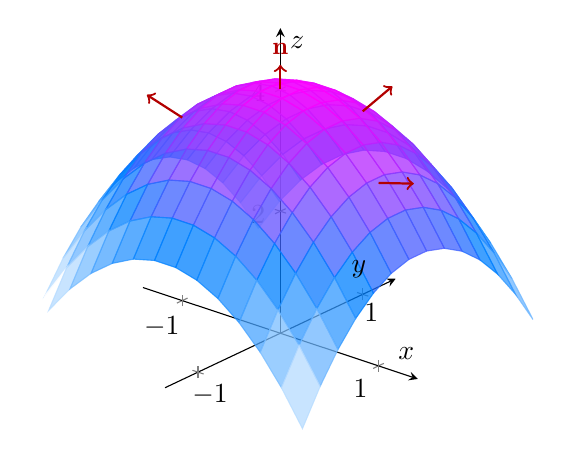
\begin{tikzpicture}
\begin{axis}[
    view={40}{25},
    xlabel={$x$}, ylabel={$y$}, zlabel={$z$},
    axis lines=center,
    tick style={thin},
    zmin=0, zmax=5,
    xtick={-1,1}, ytick={-1,1}, ztick={2,4},
    width=8cm, height=8cm,
]
    \addplot3[surf,shader=flat corner,samples=14,domain=-1.4:1.4,
              opacity=0.75,colormap/cool]{4-x^2-y^2};
    \draw[->,thick,red!70!black]
        (axis cs:1,0,3)--(axis cs:1.36,0,3.18);
    \draw[->,thick,red!70!black]
        (axis cs:0,1,3)--(axis cs:0,1.36,3.18);
    \draw[->,thick,red!70!black]
        (axis cs:-1,0,3)--(axis cs:-1.36,0,3.18);
    \draw[->,thick,red!70!black]
        (axis cs:0,0,4)--(axis cs:0,0,4.4)
        node[above]{\small $\mathbf{n}$};
\end{axis}
\end{tikzpicture}
\caption{Superficie orientada $z=4-x^2-y^2$ con vectores normales $\mathbf{n}$
         consistentes; invertir la orientación cambia el signo del flujo}
\label{fig:superficie_orientada}
\end{figure}

\begin{definition}[Flujo de un campo vectorial]
Sea $\mathbf{F}$ un campo vectorial continuo sobre una superficie orientada $S$ con normal unitaria $\mathbf{n}$. La \textbf{integral de superficie de $\mathbf{F}$ sobre $S$}, o \textbf{flujo} de $\mathbf{F}$ a través de $S$, es
\[
\iint_S \mathbf{F}\cdot\mathbf{n}\,dS.
\]
Si $S$ está parametrizada por $\mathbf{r}(u,v)$ con orientación compatible (es decir, tomando $\mathbf{n} = \frac{\mathbf{r}_u \times \mathbf{r}_v}{\|\mathbf{r}_u \times \mathbf{r}_v\|}$), entonces
\[
\iint_S \mathbf{F}\cdot\mathbf{n}\,dS
=
\iint_D \mathbf{F}\bigl(\mathbf{r}(u,v)\bigr)\cdot(\mathbf{r}_u \times \mathbf{r}_v)\,du\,dv.
\]
\end{definition}

\begin{rem}
El producto punto $\mathbf{F}\cdot\mathbf{n}$ mide cuánto del campo cruza la superficie en la dirección normal. Si es positivo, el flujo es saliente; si es negativo, entrante. La orientación de $S$ es esencial: al cambiar $\mathbf{n}$ por $-\mathbf{n}$, el flujo cambia de signo. Esta dependencia distingue a la integral vectorial de la escalar.
\end{rem}

\begin{pasos}
Para calcular el flujo de un campo vectorial a través de una superficie orientada:
\begin{enumerate}
\item \textbf{Orientar la superficie.} Decidir cuál es la normal positiva (hacia arriba, hacia afuera, o según la regla de la mano derecha).
\item \textbf{Parametrizar la superficie.} Obtener $\mathbf{r}(u,v)$ y su dominio $D$.
\item \textbf{Calcular el vector normal (no unitario).} Hallar $\mathbf{r}_u \times \mathbf{r}_v$ y verificar que su dirección coincide con la orientación elegida; si no, multiplicar por $-1$.
\item \textbf{Sustituir el campo.} Evaluar $\mathbf{F}$ en la parametrización y formar el integrando $\mathbf{F}(\mathbf{r}(u,v)) \cdot (\mathbf{r}_u \times \mathbf{r}_v)$.
\item \textbf{Evaluar la integral doble.} Integrar sobre $D$.
\end{enumerate}
\end{pasos}

% -----------------------------------------------------------
\begin{example}[Flujo a través de un cilindro]
Calcule el flujo de $\mathbf{F}(x,y,z)=\langle x,y,z\rangle$ a través de la superficie lateral del cilindro $x^2+y^2=1$, con $0\le z\le 2$, orientado hacia afuera.
\begin{myproof}
\textbf{Paso 1: Orientar la superficie.}
La normal hacia afuera en un cilindro radial apunta en la dirección de $\langle x,y,0\rangle$.

\textbf{Paso 2: Parametrizar.}
\[
\mathbf{r}(\theta,z)=\langle \cos\theta,\; \sin\theta,\; z \rangle,
\quad 0\le\theta\le 2\pi,\; 0\le z\le 2.
\]

\textbf{Paso 3: Calcular el vector normal.}
\[
\mathbf{r}_\theta = \langle -\sin\theta,\; \cos\theta,\; 0 \rangle,\quad
\mathbf{r}_z = \langle 0,\; 0,\; 1 \rangle.
\]
\[
\mathbf{r}_\theta \times \mathbf{r}_z
= \langle \cos\theta,\; \sin\theta,\; 0 \rangle.
\]
Este vector apunta hacia afuera, que es exactamente la orientación pedida.

\textbf{Paso 4: Sustituir el campo.}
Sobre el cilindro, $\mathbf{F}(\mathbf{r}(\theta,z)) = \langle \cos\theta, \sin\theta, z\rangle$. Entonces
\[
\mathbf{F}\cdot(\mathbf{r}_\theta \times \mathbf{r}_z)
= \langle \cos\theta,\sin\theta,z\rangle \cdot \langle \cos\theta,\sin\theta,0\rangle
= \cos^2\theta+\sin^2\theta = 1.
\]

\textbf{Paso 5: Evaluar la integral doble.}
\[
\iint_S \mathbf{F}\cdot\mathbf{n}\,dS
= \int_0^{2\pi}\int_0^2 1\,dz\,d\theta = 2\cdot 2\pi = 4\pi.
\]
\[
\boxed{\text{Flujo} = 4\pi}
\]
\end{myproof}
\end{example}

% -----------------------------------------------------------
\begin{example}[Flujo a través de un cono]
Calcule el flujo de $\mathbf{F}(x,y,z)=\langle 0,0,z\rangle$ a través de la superficie del cono $z=\sqrt{x^2+y^2}$, con $0\le z\le 1$, orientado hacia arriba (es decir, con componente normal positiva en $z$).
\begin{myproof}
\textbf{Paso 1: Orientar la superficie.}
La superficie es gráfica de $z=f(x,y)=\sqrt{x^2+y^2}$, con dominio $R: x^2+y^2\le 1$. La normal hacia arriba es $\mathbf{n}$ con tercera componente positiva.

\textbf{Paso 2: Parametrizar como gráfica.}
\[
\mathbf{r}(x,y)=\langle x,\; y,\; \sqrt{x^2+y^2} \rangle.
\]

\textbf{Paso 3: Calcular el vector normal.}
Sea $r=\sqrt{x^2+y^2}$. $f_x = x/r$, $f_y = y/r$. Entonces
\[
\mathbf{r}_x \times \mathbf{r}_y = \langle -x/r,\; -y/r,\; 1 \rangle.
\]
La tercera componente es $1>0$, así que coincide con la orientación pedida.

\textbf{Paso 4: Sustituir el campo.}
Sobre el cono, $\mathbf{F} = \langle 0,0,r\rangle$. Luego
\[
\mathbf{F}\cdot(\mathbf{r}_x \times \mathbf{r}_y)
= \langle 0,0,r\rangle \cdot \langle -x/r,-y/r,1\rangle = r.
\]

\textbf{Paso 5: Evaluar la integral doble.}
\[
\iint_S \mathbf{F}\cdot\mathbf{n}\,dS
= \iint_R r\,dA
= \int_0^{2\pi}\int_0^1 r\cdot r\,dr\,d\theta
= 2\pi \int_0^1 r^2\,dr
= \frac{2\pi}{3}.
\]
\[
\boxed{\text{Flujo} = \frac{2\pi}{3}}
\]
\end{myproof}
\end{example}

% ============================================================
\section{Teorema de la divergencia}
% ============================================================

El teorema de la divergencia (o teorema de Gauss) establece que el flujo total de un campo vectorial a través de la superficie cerrada que limita un sólido es igual a la integral triple de la divergencia del campo en el interior del sólido.

\begin{theorem}[Teorema de la divergencia]
Sea $Q\subset\mathbb{R}^3$ un sólido acotado con frontera suave por partes $\partial Q$, orientada con la normal unitaria exterior $\mathbf{n}$. Si $\mathbf{F}(x,y,z)$ es un campo vectorial cuyas componentes tienen derivadas parciales de primer orden continuas en $Q$, entonces
\[
\iint_{\partial Q} \mathbf{F}\cdot\mathbf{n}\,dS
=
\iiint_Q (\nabla\cdot\mathbf{F})\,dV,
\]
donde $\displaystyle \nabla\cdot\mathbf{F} = \frac{\partial P}{\partial x} + \frac{\partial Q}{\partial y} + \frac{\partial R}{\partial z}$.
\end{theorem}

\begin{rem}
La divergencia $\nabla\cdot\mathbf{F}$ mide la densidad de fuentes (positiva) o sumideros (negativa) del campo en cada punto. El teorema afirma que la cantidad neta que sale por la frontera es exactamente la suma de todas las fuentes internas. Si $\nabla\cdot\mathbf{F}=0$ en todo $Q$, el flujo neto a través de $\partial Q$ es cero: todo lo que entra, sale.
\end{rem}

\begin{proof}[Esquema de la demostración]
La demostración rigurosa sigue la misma estrategia que el Teorema Fundamental del Cálculo en una variable, aplicada a cada componente. Se divide el sólido en celdas infinitesimales y se suman los flujos; los flujos a través de las caras interiores se cancelan por pares, quedando únicamente el flujo a través de la frontera exterior. Cada celda contribuye con $\nabla\cdot\mathbf{F}\,dV$, y al tomar el límite se obtiene la integral triple. 
\par
Para la componente $P$ del campo, se aplica el teorema de Fubini y el TFC en la dirección $x$; el resultado se suma con las otras dos componentes. La orientación exterior garantiza que los signos en la frontera coincidan con los de la integral de flujo.
\end{proof}

\begin{figure}[H]
\centering
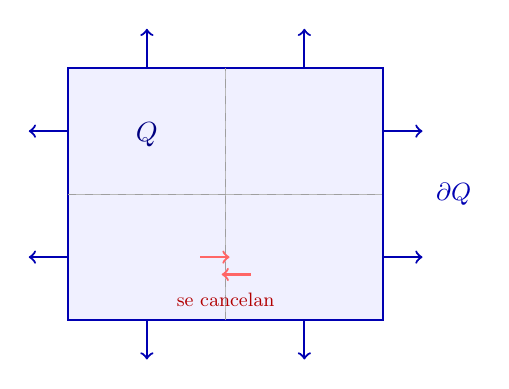
\begin{tikzpicture}[scale=1.0]
  % 2x2 grid of cells representing solid Q
  \foreach \i in {0,1} {
    \foreach \j in {0,1} {
      \fill[blue!6] (\i*2, \j*1.6) rectangle (\i*2+2, \j*1.6+1.6);
      \draw[gray!55] (\i*2, \j*1.6) rectangle (\i*2+2, \j*1.6+1.6);
    }
  }
  % Outer boundary (thick blue)
  \draw[thick, blue!70!black] (0,0) rectangle (4,3.2);
  % Interior shared faces (dashed)
  \draw[dashed, gray!75] (2,0) -- (2,3.2);
  \draw[dashed, gray!75] (0,1.6) -- (4,1.6);
  % Cancellation at interior vertical face (x=2): opposite arrows
  \draw[->, thick, red!60] (1.68, 0.80) -- (2.05, 0.80);
  \draw[<-, thick, red!60] (1.95, 0.58) -- (2.32, 0.58);
  \node[red!70!black, scale=0.78, anchor=center] at (2.0, 0.26) {\small se cancelan};
  % Outer flux arrows (outward, blue)
  \draw[->, thick, blue!70!black] (0, 0.80) -- (-0.50, 0.80);
  \draw[->, thick, blue!70!black] (0, 2.40) -- (-0.50, 2.40);
  \draw[->, thick, blue!70!black] (4, 0.80) -- ( 4.50, 0.80);
  \draw[->, thick, blue!70!black] (4, 2.40) -- ( 4.50, 2.40);
  \draw[->, thick, blue!70!black] (1, 3.2)  -- ( 1, 3.70);
  \draw[->, thick, blue!70!black] (3, 3.2)  -- ( 3, 3.70);
  \draw[->, thick, blue!70!black] (1, 0)    -- ( 1,-0.50);
  \draw[->, thick, blue!70!black] (3, 0)    -- ( 3,-0.50);
  % Labels
  \node[blue!50!black, anchor=center] at (1.0, 2.35) {$Q$};
  \node[blue!70!black, right] at (4.55, 1.6) {\small $\partial Q$};
\end{tikzpicture}
\caption{Cancelación de flujos en caras interiores (flechas rojas opuestas) en el Teorema de la Divergencia: cada cara interna tiene un flujo entrante de una celda y un flujo saliente de la celda vecina, que se anulan. Solo la frontera exterior $\partial Q$ contribuye al flujo neto (flechas azules).}
\label{fig:divergencia_cancelacion}
\end{figure}

\begin{pasos}
Para aplicar el teorema de la divergencia:
\begin{enumerate}
\item \textbf{Identificar el sólido $Q$ y su frontera $\partial Q$.} Asegurarse de que $\partial Q$ es cerrada y está orientada hacia afuera.
\item \textbf{Calcular la divergencia.} Hallar $\nabla\cdot\mathbf{F}$.
\item \textbf{Plantear la integral triple.} Escribir $\iiint_Q (\nabla\cdot\mathbf{F})\,dV$.
\item \textbf{Evaluar la integral triple.} Usar coordenadas cartesianas, cilíndricas o esféricas según la simetría del sólido.
\end{enumerate}
Si se desea verificar el teorema, también se puede calcular el flujo por separado y comparar.
\end{pasos}

% -----------------------------------------------------------
\begin{example}[Verificación del teorema de la divergencia para una esfera]
Verifique el teorema de la divergencia para $\mathbf{F}(x,y,z)=\langle x,y,z\rangle$ sobre el sólido $Q$ limitado por la esfera $x^2+y^2+z^2\le R^2$.
\begin{myproof}
\textbf{Paso 1: Identificar el sólido y la frontera.}
$Q$ es la esfera sólida de radio $R$. $\partial Q$ es la superficie esférica, orientada hacia afuera.

\textbf{Paso 2: Calcular la divergencia.}
\[
\nabla\cdot\mathbf{F} = \frac{\partial x}{\partial x}+\frac{\partial y}{\partial y}+\frac{\partial z}{\partial z} = 1+1+1=3.
\]

\textbf{Paso 3: Plantear la integral triple.}
\[
\iiint_Q 3\,dV = 3\,\text{Vol}(Q) = 3\cdot\frac{4}{3}\pi R^3 = 4\pi R^3.
\]

\textbf{Paso 4: Calcular el flujo directamente (verificación).}
Sobre la esfera, $\mathbf{n} = \frac{\langle x,y,z\rangle}{R}$ y $\mathbf{F}=\langle x,y,z\rangle$. Entonces $\mathbf{F}\cdot\mathbf{n} = \frac{x^2+y^2+z^2}{R} = R$. El flujo es
\[
\iint_{\partial Q} R\,dS = R\cdot 4\pi R^2 = 4\pi R^3.
\]
Ambos resultados coinciden.
\[
\boxed{\text{Flujo} = 4\pi R^3}
\]
\end{myproof}
\end{example}

% -----------------------------------------------------------
\begin{example}[Aplicación del teorema de la divergencia]
Calcule el flujo de $\mathbf{F}(x,y,z)=\langle y,\; xz,\; z^2\rangle$ a través de la superficie cerrada que limita el sólido $Q$ encerrado por el paraboloide $z=1-x^2-y^2$ y el plano $z=0$.
\begin{myproof}
\textbf{Paso 1: Identificar el sólido.}
$Q$ está sobre el plano $z=0$ y bajo el paraboloide $z=1-x^2-y^2$. La proyección sobre el plano $xy$ es el disco $x^2+y^2\le 1$.

\textbf{Paso 2: Calcular la divergencia.}
\[
\nabla\cdot\mathbf{F}
= \frac{\partial}{\partial x}(y) + \frac{\partial}{\partial y}(xz) + \frac{\partial}{\partial z}(z^2)
= 0 + 0 + 2z = 2z.
\]

\textbf{Paso 3: Plantear la integral triple.}
Por el teorema de la divergencia,
\[
\iint_{\partial Q}\mathbf{F}\cdot\mathbf{n}\,dS
= \iiint_Q 2z\,dV.
\]

\textbf{Paso 4: Evaluar la integral triple.}
Usamos coordenadas cilíndricas: $x=r\cos\theta$, $y=r\sin\theta$, $z=z$. El paraboloide es $z=1-r^2$, con $0\le r\le 1$, $0\le\theta\le 2\pi$, $0\le z\le 1-r^2$. El elemento de volumen es $dV = r\,dz\,dr\,d\theta$.
\[
\iiint_Q 2z\,dV
= 2\int_0^{2\pi}\int_0^1\int_0^{1-r^2} z\,r\,dz\,dr\,d\theta.
\]
Resolvemos:
\[
= 2(2\pi)\int_0^1 r\left[\frac{z^2}{2}\right]_0^{1-r^2} dr
= 2\pi\int_0^1 r(1-r^2)^2\,dr.
\]
Sea $u=1-r^2$, $du=-2r\,dr$, $r\,dr=-du/2$. Cuando $r=0$, $u=1$; cuando $r=1$, $u=0$:
\[
2\pi\int_1^0 -\frac{u^2}{2}\,du = \pi\int_0^1 u^2\,du = \frac{\pi}{3}.
\]
\[
\boxed{\text{Flujo} = \frac{\pi}{3}}
\]
\end{myproof}
\end{example}

\begin{prob}
Use el teorema de la divergencia para calcular el flujo de $\mathbf{F}(x,y,z)=\langle x^3, y^3, z^3\rangle$ a través del cubo $0\le x,y,z\le 1$.
\end{prob}

\begin{prob}
Verifique el teorema de Stokes para $\mathbf{F}(x,y,z)=\langle y, z, x\rangle$ sobre la superficie del cono $z=\sqrt{x^2+y^2}$ con $0\le z\le 1$, orientado hacia arriba.
\begin{myproof}
\textbf{Paso 1. Calcular el rotacional.}
\[
\nabla\times\mathbf{F}
=\left\langle\frac{\partial x}{\partial y}-\frac{\partial z}{\partial z},\;
\frac{\partial y}{\partial z}-\frac{\partial x}{\partial x},\;
\frac{\partial z}{\partial x}-\frac{\partial y}{\partial y}\right\rangle
=\langle0-1,\;0-1,\;0-1\rangle=\langle-1,-1,-1\rangle.
\]
\textbf{Paso 2. Integral de superficie.} Parametrizamos: $\mathbf{r}(r,\theta)=\langle r\cos\theta,r\sen\theta,r\rangle$, $r\in[0,1]$, $\theta\in[0,2\pi]$:
\[
\mathbf{r}_r\times\mathbf{r}_\theta=\langle-r\cos\theta,-r\sen\theta,r\rangle\quad(z\text{-comp.}=r>0:\text{ apunta hacia arriba}).
\]
\[
(\nabla\times\mathbf{F})\cdot(\mathbf{r}_r\times\mathbf{r}_\theta)
=\langle-1,-1,-1\rangle\cdot\langle-r\cos\theta,-r\sen\theta,r\rangle=r\cos\theta+r\sen\theta-r.
\]
\[
\iint_S(\nabla\times\mathbf{F})\cdot d\mathbf{S}
=\int_0^{2\pi}\!\int_0^1(r\cos\theta+r\sen\theta-r)\,dr\,d\theta
=\int_0^{2\pi}\frac{\cos\theta+\sen\theta-1}{2}\,d\theta
=\frac{0+0-2\pi}{2}=-\pi.
\]
\textbf{Paso 3. Verificación por integral de línea.} $\partial S$: $\mathbf{r}(t)=\langle\cos t,\sen t,1\rangle$, $d\mathbf{r}=\langle-\sen t,\cos t,0\rangle dt$, $\mathbf{F}=\langle\sen t,1,\cos t\rangle$:
\[
\oint_{\partial S}\mathbf{F}\cdot d\mathbf{r}
=\int_0^{2\pi}(-\sen^2 t+\cos t)\,dt=-\pi+0=\boxed{-\pi}.\;\checkmark
\]
\end{myproof}
\end{prob}

\begin{prob}
Calcule el flujo de $\mathbf{F}(x,y,z)=\langle 2x, -y, 3z\rangle$ a través de la esfera $x^2+y^2+z^2=4$, orientada hacia afuera.
\begin{myproof}
\textbf{Paso 1. Calcular la divergencia.}
\[
\nabla\cdot\mathbf{F}=\frac{\partial(2x)}{\partial x}+\frac{\partial(-y)}{\partial y}+\frac{\partial(3z)}{\partial z}=2-1+3=4.
\]
\textbf{Paso 2. Aplicar el teorema de la divergencia.} El sólido $Q$ es la bola de radio 2; $V=\dfrac{4}{3}\pi(2)^3=\dfrac{32\pi}{3}$.
\[
\iint_{\partial Q}\mathbf{F}\cdot\mathbf{n}\,dS=\iiint_Q 4\,dV=4\cdot\frac{32\pi}{3}=\boxed{\frac{128\pi}{3}}.
\]
\end{myproof}
\end{prob}

% ============================================================
\section{Teorema de Stokes}
% ============================================================

El teorema de Stokes generaliza el teorema de Green a superficies curvas en $\mathbb{R}^3$: relaciona la circulación de un campo vectorial a lo largo del borde de una superficie con el flujo de su rotacional a través de la superficie.

\begin{theorem}[Teorema de Stokes]
Sea $S$ una superficie orientada, suave por partes, con vector normal unitario $\mathbf{n}$, y sea $\partial S$ su curva frontera, cerrada y simple, orientada positivamente según la regla de la mano derecha (si los dedos siguen el borde, el pulgar apunta en la dirección de $\mathbf{n}$). Si $\mathbf{F}$ es un campo vectorial con derivadas parciales continuas en una región abierta que contiene a $S$, entonces
\[
\oint_{\partial S} \mathbf{F}\cdot d\mathbf{r}
=
\iint_S (\nabla\times\mathbf{F})\cdot\mathbf{n}\,dS,
\]
donde $\displaystyle \nabla\times\mathbf{F} = \left( \frac{\partial R}{\partial y}-\frac{\partial Q}{\partial z},\; \frac{\partial P}{\partial z}-\frac{\partial R}{\partial x},\; \frac{\partial Q}{\partial x}-\frac{\partial P}{\partial y} \right)$.
\end{theorem}

\begin{rem}
La interpretación física es clara: la circulación total del campo alrededor del borde de una superficie es igual a la suma de las ``micro-circulaciones'' (el rotacional) a través de la superficie. Si $\nabla\times\mathbf{F}=\mathbf{0}$ en toda la superficie, el campo es irrotacional y la integral de línea sobre cualquier curva cerrada que limite una porción de $S$ es cero (independencia de la trayectoria local).
\end{rem}

\begin{figure}[H]
\centering
\begin{tikzpicture}[scale=1.1]
  % Surface S (closed organic shape suggesting a curved surface)
  \fill[green!8]
    (-2,0) to[out=70,in=190] (0,1.8) to[out=10,in=100] (2.2,0.5)
           to[out=280,in=0]  (0,-1.4) to[out=180,in=270] cycle;
  % Boundary ∂S with right-hand rule orientation (arrows)
  \draw[thick, red!70!black,
        postaction={decorate, decoration={markings,
          mark=at position 0.12 with {\arrow[red!70!black]{stealth}},
          mark=at position 0.42 with {\arrow[red!70!black]{stealth}},
          mark=at position 0.72 with {\arrow[red!70!black]{stealth}}}}]
    (-2,0) to[out=70,in=190] (0,1.8) to[out=10,in=100] (2.2,0.5)
           to[out=280,in=0]  (0,-1.4) to[out=180,in=270] cycle;
  % Normal vectors n on surface
  \draw[->, thick, blue!70!black] (-0.8,0.4) -- (-0.4,1.2)
        node[left] {\small $\mathbf{n}$};
  \draw[->, thick, blue!70!black] ( 0.6,0.2) -- ( 1.0,1.0);
  \draw[->, thick, blue!70!black] ( 1.6,0.4) -- ( 2.0,1.2);
  % Micro-circulations (small CCW arcs on surface patches)
  \foreach \cx/\cy in {-0.8/-0.2, 0.3/0.7, 1.1/-0.3} {
    \draw[->, gray!60, thin] (\cx,\cy) arc[start angle=0, end angle=300, radius=0.22];
  }
  % Labels
  \node[green!40!black, anchor=center] at (0.3,-0.2) {$S$};
  \node[red!70!black, below] at (0,-1.6) {\small $\partial S$};
  \node[gray!55, scale=0.82, anchor=east] at (-1.6,-0.7) {\small micro-circulaciones};
  \draw[->, gray!45, thin] (-1.0,-0.65) -- (-0.6,-0.2);
\end{tikzpicture}
\caption{Superficie orientada $S$ con borde $\partial S$ (rojo): la orientación de $\partial S$ sigue la regla de la mano derecha respecto de $\mathbf{n}$. Las micro-circulaciones del rotacional (arcos grises) se cancelan entre parches adyacentes; al sumar sobre toda $S$, solo queda la circulación total sobre $\partial S$.}
\label{fig:stokes_superficie}
\end{figure}

\begin{proof}[El teorema de Green como caso particular de Stokes]
Si la superficie $S$ es una región plana en el plano $xy$, podemos parametrizarla como $\mathbf{r}(x,y)=\langle x,y,0\rangle$ con $(x,y)\in R$. Su normal es $\mathbf{n}=\mathbf{k}$, y el borde $\partial S$ es la curva cerrada que limita a $R$ en el plano. 
\par
El teorema de Stokes se convierte en
\[
\oint_{\partial S} \mathbf{F}\cdot d\mathbf{r}
=
\iint_R (\nabla\times\mathbf{F})\cdot\mathbf{k}\,dA.
\]
Escribamos $\mathbf{F}(x,y,z)=\langle P(x,y), Q(x,y), 0\rangle$. Entonces
\[
\nabla\times\mathbf{F}
=
\left\langle 0,\; 0,\; \frac{\partial Q}{\partial x}-\frac{\partial P}{\partial y} \right\rangle.
\]
El producto con $\mathbf{k}$ da $\frac{\partial Q}{\partial x}-\frac{\partial P}{\partial y}$. Por tanto,
\[
\oint_{\partial S} \mathbf{F}\cdot d\mathbf{r}
=
\iint_R \left( \frac{\partial Q}{\partial x}-\frac{\partial P}{\partial y} \right)dA,
\]
que es exactamente la forma vectorial del teorema de Green estudiada en L4.1. Esta demostración muestra que Stokes es una generalización natural de Green al incorporar superficies curvas y campos tridimensionales.
\end{proof}

\begin{pasos}
Para aplicar el teorema de Stokes:
\begin{enumerate}
\item \textbf{Identificar la superficie $S$ y su borde $\partial S$.} Asegurarse de que la orientación del borde es compatible con la normal de $S$ (regla de la mano derecha).
\item \textbf{Calcular el rotacional.} Hallar $\nabla\times\mathbf{F}$.
\item \textbf{Escoger el lado más simple.} Decidir si es más fácil calcular la integral de línea sobre $\partial S$ o la integral de superficie del rotacional.
\item \textbf{Parametrizar y evaluar.} Si se usa la superficie, calcular $dS$ y $\mathbf{n}$; si se usa el borde, parametrizar la curva.
\end{enumerate}
\end{pasos}

% -----------------------------------------------------------
\begin{example}[Verificación de Stokes para un paraboloide]
Verifique el teorema de Stokes para $\mathbf{F}(x,y,z)=\langle -y,\; x,\; z\rangle$ sobre la superficie $S: z=4-x^2-y^2$, con $z\ge 0$ (orientada hacia arriba).
\begin{myproof}
\textbf{Paso 1: Identificar superficie y borde.}
La proyección de $S$ es el disco $x^2+y^2\le 4$. El borde $\partial S$ es la circunferencia $x^2+y^2=4$, $z=0$, orientada positivamente vista desde arriba (es decir, en sentido antihorario).

\textbf{Paso 2: Calcular el rotacional.}
\[
\nabla\times\mathbf{F}
=
\left\langle
\frac{\partial z}{\partial y}-\frac{\partial x}{\partial z},\;
\frac{\partial (-y)}{\partial z}-\frac{\partial z}{\partial x},\;
\frac{\partial x}{\partial x}-\frac{\partial (-y)}{\partial y}
\right\rangle
=
\langle 0-0,\;0-0,\;1-(-1)\rangle
=
\langle 0,0,2\rangle.
\]

\textbf{Paso 3: Calcular la integral de superficie (lado izquierdo de Stokes).}
Para la gráfica $z=f(x,y)$, $\mathbf{r}_x\times\mathbf{r}_y=\langle -f_x,-f_y,1\rangle$. Aquí $f_x=-2x, f_y=-2y$, así que la normal hacia arriba es $\langle 2x,2y,1\rangle$ (sin normalizar, pues $dS$ se combina con la norma). Entonces
\[
(\nabla\times\mathbf{F})\cdot(\mathbf{r}_x\times\mathbf{r}_y)
= \langle 0,0,2\rangle\cdot\langle 2x,2y,1\rangle = 2.
\]
La integral es
\[
\iint_S (\nabla\times\mathbf{F})\cdot\mathbf{n}\,dS
= \iint_R 2\,dA = 2\cdot \pi(2)^2 = 8\pi.
\]

\textbf{Paso 4: Calcular la integral de línea (verificación).}
Parametrizamos el borde: $\mathbf{r}(t)=\langle 2\cos t, 2\sin t, 0\rangle$, $0\le t\le 2\pi$. Entonces $\mathbf{F}=\langle -2\sin t, 2\cos t, 0\rangle$, $d\mathbf{r}=\langle -2\sin t, 2\cos t, 0\rangle dt$. El producto punto es
\[
(-2\sin t)(-2\sin t) + (2\cos t)(2\cos t) = 4\sin^2 t + 4\cos^2 t = 4.
\]
Luego
\[
\oint_{\partial S}\mathbf{F}\cdot d\mathbf{r} = \int_0^{2\pi} 4\,dt = 8\pi.
\]
Ambos resultados coinciden.
\[
\boxed{8\pi}
\]
\end{myproof}
\end{example}

% -----------------------------------------------------------
\begin{example}[Aplicación de Stokes a un hemisferio]
Calcule $\displaystyle \oint_C \mathbf{F}\cdot d\mathbf{r}$, donde $\mathbf{F}(x,y,z)=\langle z,\; x,\; y\rangle$ y $C$ es la curva $x^2+y^2=1$, $z=0$, recorrida en sentido antihorario vista desde arriba.
\begin{myproof}
\textbf{Paso 1: Identificar superficie y borde.}
La curva $C$ es el borde del hemisferio superior $S: x^2+y^2+z^2=1$, $z\ge 0$, orientado con normal hacia arriba (la normal exterior a la esfera tiene componente $z$ positiva en el hemisferio superior).

\textbf{Paso 2: Calcular el rotacional.}
\[
\nabla\times\mathbf{F}
=
\left\langle
\frac{\partial y}{\partial y}-\frac{\partial x}{\partial z},\;
\frac{\partial z}{\partial z}-\frac{\partial y}{\partial x},\;
\frac{\partial x}{\partial x}-\frac{\partial z}{\partial y}
\right\rangle
=
\langle 1-0,\;1-0,\;1-0\rangle
=
\langle 1,1,1\rangle.
\]

\textbf{Paso 3: Calcular la integral de superficie.}
Sobre el hemisferio, la normal exterior unitaria es $\mathbf{n}=\langle x,y,z\rangle$. Entonces
\[
(\nabla\times\mathbf{F})\cdot\mathbf{n} = \langle 1,1,1\rangle\cdot\langle x,y,z\rangle = x+y+z.
\]
Por simetría, $\iint_S x\,dS = \iint_S y\,dS = 0$ (la región es simétrica respecto a los planos $x=0$ e $y=0$, y los integrandos son impares). Queda
\[
\iint_S z\,dS.
\]
Usamos coordenadas esféricas para el hemisferio de radio 1: $z=\cos\phi$, $dS=\sin\phi\,d\phi\,d\theta$, con $\phi\in[0,\pi/2]$, $\theta\in[0,2\pi]$.
\[
\iint_S z\,dS
= \int_0^{2\pi}\int_0^{\pi/2} \cos\phi\sin\phi\,d\phi\,d\theta
= 2\pi \cdot \frac{1}{2} = \pi.
\]
Por tanto, el flujo del rotacional es $\pi$.

\textbf{Paso 4: Conclusión por Stokes.}
\[
\oint_C \mathbf{F}\cdot d\mathbf{r} = \pi.
\]
\[
\boxed{\pi}
\]
\end{myproof}
\end{example}

% ============================================================
\section{Problemas propuestos}
% ============================================================
\begin{prob}
Un campo de fuerzas $\mathbf{F}(x,y) = \langle e^x \cos y + y,
-e^x \sin y + x \rangle$ actúa sobre una partícula.
\begin{enumerate}[(a)]
    \item Demuestre que $\mathbf{F}$ es conservativo.
    \item Encuentre la función potencial $f$.
    \item Calcule el trabajo realizado por $\mathbf{F}$ al mover una
    partícula desde $(0,0)$ hasta $(1,\pi/2)$.
\end{enumerate}
\end{prob}

\begin{prob}
Verifique el teorema de Green para el campo $\mathbf{F}(x,y) =
\langle x^2 y, x y^2 \rangle$ y el rectángulo $0\le x\le 2$,
$0\le y\le 1$.
\end{prob}

\begin{prob}
Use el teorema de Green para calcular
\[
\oint_C (x^2 + y^2)\,dx + (2xy)\,dy,
\]
donde $C$ es el cuadrado con vértices $(0,0)$, $(2,0)$, $(2,2)$,
$(0,2)$ orientado positivamente.
\end{prob}

\begin{prob}
Calcule la integral de línea
\[
\oint_C -y^3\,dx + x^3\,dy
\]
donde $C$ es el círculo $x^2+y^2=4$ orientado positivamente, usando
el teorema de Green. Compare con la evaluación directa.
\end{prob}


\begin{prob}
Calcule $\displaystyle \iint_S xy\,dS$, donde $S$ es la porción del cilindro $x^2+z^2=1$ con $y\ge 0$, $z\ge 0$.
\end{prob}

\begin{prob}
Halle el área de la superficie del toro generado al rotar la circunferencia $(x-2)^2+z^2=1$ alrededor del eje $z$.
\end{prob}

\begin{prob}
Calcule la divergencia y el rotacional de los siguientes campos:
\begin{multicols}{2}
\begin{enumerate}[(a)]
    \item $\mathbf{F}(x,y,z)=\langle x^2, y^2, z^2 \rangle$
    \item $\mathbf{F}(x,y,z)=\langle yz, xz, xy \rangle$
    \item $\mathbf{F}(x,y,z)=\langle e^x, \sin y, \cos z \rangle$
    \item $\mathbf{F}(x,y,z)=\langle -y, x, 0 \rangle$
\end{enumerate}
\end{multicols}
\end{prob}

\begin{prob}
Demuestre que para cualquier campo $\mathbf{F}$ con segundas derivadas
parciales continuas, se cumple $\nabla \cdot (\nabla \times \mathbf{F})
= 0$. Esto muestra que el rotacional de un campo siempre es
\emph{solenoidal} (sin divergencia). Use un ejemplo concreto para
verificar esta identidad.
\end{prob}

\begin{prob}
Interprete físicamente el resultado del problema anterior:
si $\mathbf{F}$ es el campo de velocidades de un fluido, ¿qué significa
que $\nabla \cdot (\nabla \times \mathbf{F})=0$?
\end{prob}



\begin{prob}
Una lámina tiene la forma de la superficie $z=xy$ sobre el cuadrado $0\le x\le 2$, $0\le y\le 2$. Su densidad superficial es $\rho=x^2+y^2$. Halle su masa y su centro de masa.
\end{prob}



\begin{prob}
Sea $\mathbf{F}(x,y,z)=\langle -y, x, 2z\rangle$. Calcule la circulación de $\mathbf{F}$ alrededor del cuadrado en el plano $z=1$ con vértices $(1,1,1),(-1,1,1),(-1,-1,1),(1,-1,1)$.
\end{prob}



\begin{prob}
Demuestre que si $\mathbf{F}$ es un campo conservativo (es decir, $\mathbf{F}=\nabla f$), entonces $\nabla\times\mathbf{F}=0$ y su flujo a través de cualquier superficie cerrada es cero (por el teorema de la divergencia) y su circulación a través de cualquier borde cerrado es cero (por Stokes).
\end{prob}

\begin{prob}
Calcule el flujo de $\mathbf{F}(x,y,z)=\langle x, y, z\rangle$ a través del sólido $Q$ limitado por el paraboloide $z=4-x^2-y^2$ y el plano $z=0$.
\end{prob}

\begin{prob}
Considere el campo vectorial $\mathbf{F}=\left(6xy^3+2z^2\right)\mathbf{i}+\left(9x^2y^2\right)\mathbf{j}+\left(4xz+1\right)\mathbf{k}$. Determine si es un campo vectorial conservativo, y si lo es calcule su función potencial.
\end{prob}

\begin{prob}
Calcule la integral $\displaystyle\int_{C}(8x+36z)\,ds$ donde $C$ es la curva $x=t$, $y=t^2$, $z=t^3$ con $0\leq t\leq 2$.
\end{prob}

\begin{prob}
Calcule la integral $\displaystyle\int_{C}(\cos x+2yz)\,dx+(\sen y+2xz)\,dy+(z+2xy)\,dz$ en el segmento de recta del punto $(0,0,0)$ a $(\pi,\pi,0)$.
\end{prob}
